\section{Potential Future Development}

This section presents two core future expansion directions aimed at improving extensibility, personalizing the user experience, and supporting user-generated content.

\vspace{0.5cm}

\subsection{Future Direction 1: In-Game Custom Map Builder}

\subsubsection{Functional Overview}
This feature allows players to directly design 2D maps within the game interface:
\begin{itemize}
    \item Placement and removal of terrain blocks, functional blocks (\texttt{QuestionBlock}, \texttt{BrickBlock}, \texttt{Lifter}), items, enemy spawn locations (\texttt{Goomba}, \texttt{Koopa}, \texttt{Witch}, \texttt{ThorKing}), player spawn points, and destinations (\texttt{Flag}, \texttt{Princess}).
    \item Support for undo/redo operations, visual theme selection (Overworld, Underground, Castle), JSON map saving/exporting, and an instant playtest mode.
\end{itemize}

\subsubsection{Evaluation of the Current Design (OOP/SOLID Perspective)}
\textbf{Strengths (Reusability):}
\begin{itemize}
    \item The \texttt{MapData} data structure cleanly separates the tile grid layer (\texttt{TileLayer}) from the entity list (\texttt{ObjectLayer}), making it suitable as an in-memory map representation.
    \item The \texttt{LevelManager} already provides validation and update operations through \texttt{setTileID()}, along with a \texttt{VertexArray}-based batch rendering mechanism.
    \item The \texttt{LevelBuilder} and existing factories (\texttt{HeroFactory}, \texttt{BlockFactory}, \texttt{EnemyFactory}) can be reused to build a \texttt{GameWorld} from \texttt{MapData}, providing a foundation for the playtest feature.
\end{itemize}

\vspace{0.3cm}
\noindent\textbf{Weaknesses and Design Challenges (OOP/SOLID):}
\begin{itemize}
    \item \textbf{Potential Single Responsibility Principle (SRP) Violation:} If a single \texttt{MapEditorState} class is implemented to handle mouse input, UI palettes, tile-map modification, JSON serialization, and history management, it could accumulate too many responsibilities and become a God Object.
    
    \item \textbf{Limited Extensibility of Entity Registration:} Currently, entity classification in the \texttt{LevelBuilder} relies on string comparisons (e.g., \texttt{className == "goomba"}). Applying the same approach to the editor toolbar would require modifying the editor source code whenever a new entity type is introduced, limiting compliance with the Open-Closed Principle (OCP).
    
    \item \textbf{Missing Serialization Support:} The \texttt{MapManager} currently provides map loading through \texttt{loadMap()}, but does not support serializing modified map data back into the expected JSON/Tiled Map format.
\end{itemize}

\subsubsection{Proposed Architecture}
\begin{itemize}
    \item \textbf{Command Pattern (\texttt{IEditorCommand}):} Encapsulates each editing operation (e.g., placing/removing a tile, adding/removing an enemy) into command objects supporting \texttt{execute()} and \texttt{undo()}, enabling safe Undo/Redo functionality while keeping history management separate from the editor state.
    
    \item \textbf{Strategy Pattern (\texttt{IEditorTool}):} Separates editor interaction modes (\texttt{TileBrushTool}, \texttt{EraserTool}, \texttt{EntityTool}) into independent and interchangeable tool strategies.
    
    \item \textbf{Dedicated \texttt{MapSerializer}:} Separates map validation and serialization responsibilities by validating \texttt{MapData} through operations such as \texttt{validateMap()} and converting it into the required JSON format.
\end{itemize}

\begin{figure}[h]
\centering
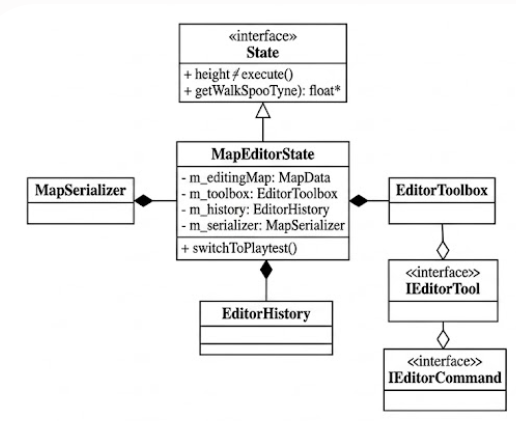
\includegraphics[width=0.45\textwidth]{img/future_suggestion_1.png}
\caption{Proposed Architecture for In-Game Map Builder}
\end{figure}

\FloatBarrier

\subsection{Future Direction 2: Data-Driven Gameplay Configuration}

\subsubsection{Functional Overview}
This feature allows players or developers to directly customize runtime gameplay parameters:
\begin{itemize}
    \item \textbf{Hero Parameters:} Walking speed, jump force, acceleration, invincibility duration, special-skill cooldown, and initial life count.
    \item \textbf{Enemy Parameters:} Maximum health, patrol speed, movement range, and attack frequency for bosses and witches.
    \item \textbf{World Physics Parameters:} Global gravity, friction coefficients, and maximum fall speed.
    \item \textbf{Preset Profile System:} Provides predefined modes (\textit{Classic}, \textit{Moon Jump -- Low Gravity}, \textit{Turbo Speedrun}, \textit{Nightmare Hardcore}) and supports saving or sharing configuration profiles in JSON format.
\end{itemize}

\subsubsection{Evaluation of the Current Design (OOP/SOLID Perspective)}
\textbf{Strengths (Reusability):}
\begin{itemize}
    \item The separation between character states (\texttt{HeroState}) and the physics system (\texttt{WorldPhysicsSystem}) already encapsulates movement and physics calculations within dedicated components.
    
    \item The project has already integrated the \texttt{nlohmann::json} library within the \texttt{SaveManager}, providing an existing foundation for implementing a gameplay configuration parser.
    
    \item The \texttt{SettingsState} already contains a slider-based UI component (\texttt{VolumeSlider}), which can be reused as a basis for implementing parameter controls in a \texttt{CustomizationState}.
\end{itemize}

\vspace{0.3cm}
\noindent\textbf{Weaknesses and Design Challenges (OOP/SOLID):}
\begin{itemize}
    \item \textbf{Compile-Time Configuration Coupling:} State classes such as \texttt{RunState} and \texttt{JumpState} directly depend on compile-time constants defined in \texttt{PhysicsConstants.h} (e.g., \texttt{constexpr float WALK\_SPEED}, \texttt{JUMP\_FORCE}). This tightly couples gameplay behavior to a fixed parameter set.
    
    \item \textbf{Limited Runtime Configurability:} Rebalancing the game or experimenting with alternative parameter values currently requires modifying the C++ source code and recompiling the application.
    
    \item \textbf{Hardcoded Gameplay Parameters:} Several enemy and physics parameters, such as enemy speed and gravity (\texttt{1500.f}), are directly embedded within components such as \texttt{EnemyFactory} and \texttt{WorldPhysicsSystem}.
\end{itemize}

\subsubsection{Proposed Architecture}
\begin{itemize}
    \item \textbf{Data-Driven Configuration System:} Moves gameplay constants into dedicated configuration objects (\texttt{HeroStatsConfig}, \texttt{EnemyStatsConfig}, \texttt{WorldPhysicsConfig}) that are dynamically loaded from a \texttt{config/gameplay.json} file through the \texttt{GameConfigRegistry}.
    
    \item \textbf{Provider-Based Dependency Injection:} Gameplay systems obtain configuration data through abstractions such as \texttt{IStatsProvider} and \texttt{IPhysicsConfigProvider} rather than directly accessing global or compile-time constants.
    
    \item \textbf{\texttt{CustomizationState}:} Provides sliders and other UI controls for modifying configuration values in memory before applying them to the active \texttt{LevelRuntime}.
\end{itemize}

\begin{figure}[h]
\centering
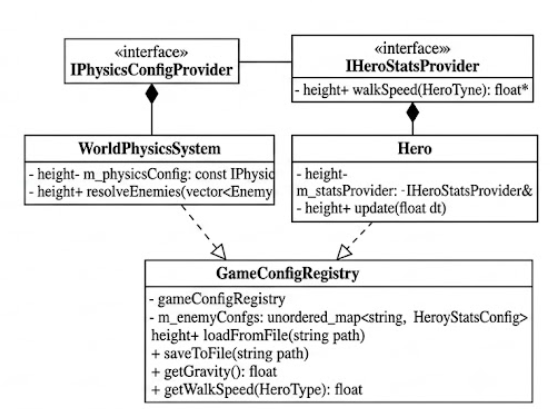
\includegraphics[width=0.45\textwidth]{img/future_suggestion_2.png}
\caption{Proposed Architecture for Data-Driven Gameplay Configuration}
\end{figure}